\begin{figure}[!ht]
 \centering
 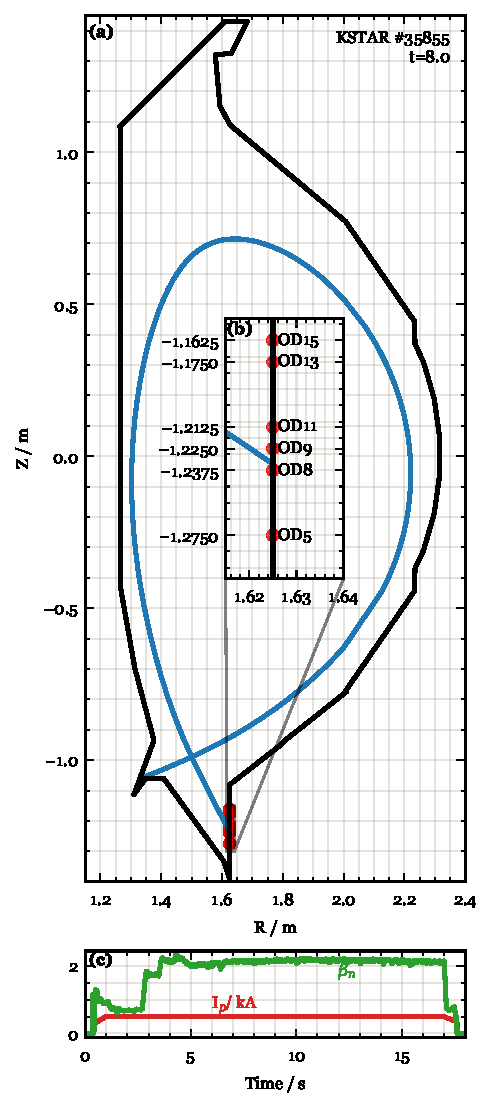
\includegraphics[width=\linewidth]{figures/RefShot.pdf}
 \caption{
Reference shot \#35851.
(a) Showing last closed flux surface at t=8 seconds.
The magnetic shape control was programmed to keep X point fixed which provided a sufficiently stable strike point on the realtime Langmuir Probe array.
(b) Zoomed-in locations of realtime Outer Divertor (OD) Langmuir probes.
(c) Plasma current (I$_p$) and $\beta_n$ for reference shot.
}
 \label{fig:ref_shot}
\end{figure}

\section{Experimental setup and control variables}
\label{sec:control_variables}

\begin{figure}[!ht]
 \centering
 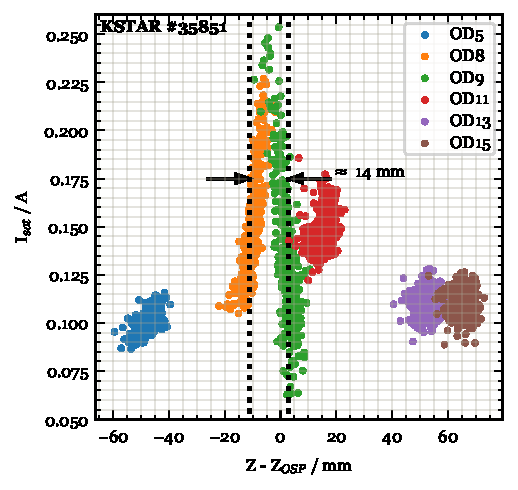
\includegraphics[width=\linewidth]{figures/StrikePointWidth.pdf}
 \caption{
Strike point width estimation for reference shot \# 35851.
the raw data from langmuir probe array has been filtered by 8th order Butterworth filter ith cut-off frequency of 20 Hz and then down sampled to 40 Hz.
For each data point on this plot, the x-axis position is calculated by subtracting the \ac{OSP} position reported by EFIT from the probe's Z coordinate.
}
 \label{fig:strike_point_width}
\end{figure}

The experiment was conducted on a standard lower single null H-mode plasma profile with reference shot KSTAR \#35851 with the equilibrium profile as shown in Fig.\ref{fig:ref_shot}.
The plasma shaping steps commenced by 7~s and the shot was programmed for flat-top up to 17~s providing a 10~s long window for the detachment control experiment.
For heat flux control, N$_2$ gas puffing was used.
The heat flux control variable was tested with several different inputs.

First, we utilized previously developed \ac{Afrac}\cite{Eldon_2022_PPCF}, which is defined as the ratio of measured ion saturation current ($I_{sat, measured}$) to modeled (using 2PM\cite{Leonard_2018_PPCF}) ion saturation current assuming fully attachment plasma ($I_{sat, attached}$).
\begin{equation}
    A_{frac} = \frac{I_{sat, measured}}{I_{sat, attached}}
\end{equation}

$I_{sat, attached}$ is estimated using Eq.(13) from \cite{Eldon_2022_PPCF}:

\begin{equation}
    I_{sat, attached} = C \langle n_{e} \rangle^2 q_{||, a}^{-\frac{3}{7}} 
\end{equation}

Here, $C$ is a calibration constant determined during reference shots so that \ac{Afrac} is 1.0 when \ac{SOL} plasma is fully attached to the divertor, $\langle n_{e} \rangle$ is the line-averaged electron density measured by interferometer and $q_{||, a}$ is the heat flux density at the outer mid-plane which is estimated using Eq.(15) from \cite{Eldon_2022_PPCF}.
The calibration constant $C$ accounts for gaps in real-time data availability on KSTAR and may be removed if more measurements become available in the future.
\ac{Afrac} is a convenient choice of control variable that is easily available in most tokamaks and allows for cross-comparison among machines.
If the strike point on the divertor tile is fixed in position well enough by the shape control system, a single close-by Langmuir probe is enough to provide the ion saturation current required for \ac{Afrac} calculation.
However, if the strike point control is not good enough, or if it is required to leave it as a free variable to allow for controlling other parameters in the shape control loop (as was the case in our experiments), then it is required to estimate the true ion saturation current through measurements made by a Langmuir probe array.
In our experiments, we chose the peak value from the Langmuir probe array as the input to the ion saturation current at the strike point.
Fig.\ref{fig:strike_point_width} plots the data from this Langmuir probe array for our reference shot.
The horizontal axis in this figure has been referenced from the EFIT reported \ac{OSP} position.
Thus, this figure shows the spread of the ion saturation current profile across the strike point.
Here, we see that the strike point is closer to OD8 and OD9 with a peak ion saturation current value of roughly 0.2~A at the strike point position.
We estimate the width of the ion saturation current profile at half the maximum value referenced to the baseline value of 0.05~A measured by far away probes, giving FWHM$\gtrsim$16~mm.
This ensures that when the strike point is within the closely placed probes, OD8, OD9, and OD11 (Fig.\ref{fig:ref_shot}), at least one probe can measure the ion saturation current while being within the peak region of the strike point.
We used the maximum value measured among the probe array to calculate \ac{Afrac} and since these probes are 12.5~mm apart, it means that the maximum deviation from the actual peak value would be $\lesssim$35\%.
Assuming that the strike point stays for equal amount of time in any location between the probe array (uniformly distributed, this can be further corraborated by noticing the motion of strike point in the figures in later sections), the mean error in peak value would be about 13\% while median error would be about 10\% assuming a gaussian profile with 16~mm FWHM.
This estimation in turn sets goals for a potential future strike point controller, to bound the strike point movement within 6.25~mm of the probe location to achieve above mentioned uncertainties.
If such a strike point controller can keep the strike point motion within 2.35~mm, the mean error would go below 2\% which would already be better than the other sources of error in the ion saturation current measurement.

Langmuir probes would not be able to survive high heat flux in burning plasma future reactors.
In general, such reactors would be severely limited in the number of realtime sensors available for control systems because of high neutron fluence and heat flux in vacuum vessels, and thus alternate control variables need to be searched for.
Toward this goal, we tested a prototype of a machine-learning-based surrogate model of 2D UEDGE, DivControlNN.
The employed version of DivControlNN is trained on approximately 70,000 2D UEDGE simulations of KSTAR.
The training dataset scanned core electron density ($1.5 \times 10^{19} - 7.0 \times 10^{19}$ m$^{-3}$), plasma current ($600-800$ kA), total input power split evenly between ion and electron channels ($1-8$ MW), impurity fraction with respect to Deuterium density ($0-0.04$), and scaling of diffusion coefficient profile with a factor ($0.6 - 2$).
The diffusion coefficient profile is assumed for a typical H-mode shot which can be scaled as an input to the model.
This provided a widely applicable surrogate model that gives steady-state values of heat flux, ion saturation current, and electron temperature along the two divertors, electron density and temperature at the upstream point of the midplane, and total radiated power, power fraction radiated from divertor, and peak radiation power location in the poloidal cross-section of the device.
The model generates output within 20\% error from the 2D UEDGE output.

DivControlNN was originally developed and trained using Python's TensorFlow package and consists of two different models working in tandem.
The first is a multi-modal $\beta$-variational autoencoder\cite{Higgins_2017_ICLR} model to compress various quantities of interest coming from synthetic diagnostics on a 2D UEDGE database into a latent space representation.
The second stage is a multi-layer perceptron (MLP) model that maps the inputs of the 2D UEDGE simulations (which also form the inputs to the overall surrogate model).
During inference operation, the MLP model first maps the inputs to the latent space and the decoder network from the autoencoder then decodes the latent space into useful outputs.
While Python is the industry choice for developing and training such models, it can not be used for real-time inference purposes such as our use case.
We converted the Python model into a pure C code using a keras2c\cite{keras2c} package which is developed for generally converting such neural networks into real-time compatible C codes.
The generated C code runs an inference operation in about 160 $\mu$s on Intel\textsuperscript{\textregistered} Core\textsuperscript{TM} i7-6600U CPU @ 2.60GHz while we saw speed up of up to 18 $\mu$s per inference on Apple\textsuperscript{\textregistered} M2\textsuperscript{TM} Pro.
The real-time PCS in KSTAR runs its divertor control categories in a 50 $\mu$s clock cycle CPU, so we ran DivControlNN in a separate 1 ms clock-cycle CPU ensuring enough runtime for it along with other processes in that CPU.
This was still more than sufficient for our control purposes which anyway can not control faster than a few 10s of Hz due to system response time and gas actuation speed.

This preliminary model, however, has been trained on 2D UEDGE simulations of KSTAR with carbon divertor and carbon as the sole impurity species.
So the model does not exactly capture the environment with tungsten impurity from the tungsten divertor it was tested in, however the radiation loss profiles due to carbon and nitrogen (which was used in the test) are sufficiently similar to expect ballpark accuracy at the very least.
So it does not reflect the same Tungsten divertor system in which it was tested.
There were several other limitations to the realtime input provided to the model.
There was no reliable input for impurity fraction in plasma and we created an ad-hoc gas accumulation model which estimated impurity fraction by taking the ratio of total puffed impurity with total puffed Deuterium gas with estimated decay rates to model the effect of pumping and wall adsorption.
It turned out that even this estimator did not work correctly during the shots and we discuss this more in Sec.\ref{sec:sysid} later.
Additionally at KSTAR, the total input power from NBI and ECH sources is not completely available in realtime PCS and we had to input a feedforward signal matching the programmed rate of some sources that got summed with the other sources whose power was available in realtime.
Such feedforward programming is vulnerable to changes in actal power delivered during the shot including timing mismatch of on/off commands of NBI sources as well as power drop out when a source fails during the shot.
The ohmic power contribution is also prone to errors as a simple production $P_{ohm} \approx I_p \cdot V_{loop}$ is used in realtime estimate which assumes that all $I_p$ is inductively driven and ignores current drive due to other sources.
Finally, the diffusion coefficient scaling factor was set to 1.0 for lack of any better realtime information on it.
Despite these limitations, we attempted to use this model as a preliminary test for using such a surrogate model in real time and identify major obstacles before testing an improved and more relevant version in the future.
